\documentclass[a4paper, 11pt]{article} % Uses article class in A4 format

%----------------------------------------------------------------------------------------
%	FORMATTING
%----------------------------------------------------------------------------------------

\addtolength{\hoffset}{-2.25cm}
\addtolength{\textwidth}{4.5cm}
\addtolength{\voffset}{-3.25cm}
\addtolength{\textheight}{5cm}
\setlength{\parskip}{0pt}
\setlength{\parindent}{0in}

%----------------------------------------------------------------------------------------
%	PACKAGES AND OTHER DOCUMENT CONFIGURATIONS
%----------------------------------------------------------------------------------------

\usepackage{charter} % Use the Charter font
\usepackage[utf8]{inputenc} % Use UTF-8 encoding
\usepackage{microtype} % Slightly tweak font spacing for aesthetics

\usepackage[english]{babel} % Language hyphenation and typographical rules

\usepackage{tabularx}
\usepackage{amsthm, amsmath, amssymb} % Mathematical typesetting
\usepackage{float} % Improved interface for floating objects
\usepackage[final, colorlinks = true, 
linkcolor = black, 
citecolor = black]{hyperref} % For hyperlinks in the PDF
\usepackage{graphicx, multicol} % Enhanced support for graphics
\usepackage{color}
\usepackage{xcolor} % Driver-independent color extensions
\usepackage{marvosym, wasysym} % More symbols
\usepackage{rotating} % Rotation tools
\usepackage{censor} % Facilities for controlling restricted text
\usepackage{listings, lstautogobble} % Environment for non-formatted code
\usepackage{pseudocode} % Environment for specifying algorithms in a natural way
\usepackage{algorithm}
\usepackage{algpseudocode}
\renewcommand{\algorithmicrequire}{\textbf{Input:}}
\renewcommand{\algorithmicensure}{\textbf{Output:}}
\usepackage{booktabs} % Enhances quality of tables

\usepackage{cases}
\usepackage{bookmark}

\usepackage{tikz-qtree} % Easy tree drawing tool
\tikzset{every tree node/.style={align=center,anchor=north},
	level distance=2cm} % Configuration for q-trees

\usepackage[backend=biber,style=numeric,
sorting=nyt]{biblatex} % Complete reimplementation of bibliographic facilities

\usepackage{csquotes} % Context sensitive quotation facilities

\usepackage[yyyymmdd]{datetime} % Uses YEAR-MONTH-DAY format for dates
\renewcommand{\dateseparator}{-} % Sets dateseparator to '-'

\usepackage{fancyhdr} % Headers and footers
\pagestyle{fancy} % All pages have headers and footers
\fancyhead{}\renewcommand{\headrulewidth}{0pt} % Blank out the default header
\fancyfoot[L]{} % Custom footer text
\fancyfoot[C]{} % Custom footer text
\fancyfoot[R]{\thepage} % Custom footer text

\newcommand{\note}[1]{\marginpar{\scriptsize \textcolor{red}{#1}}} % Enables comments in red on margin

\usepackage{fontspec}
\setmonofont{Consolas}
\definecolor{codegreen}{rgb}{0,0.6,0}
\definecolor{codegray}{rgb}{0.5,0.5,0.5}
\definecolor{codemauve}{rgb}{0.58,0,0.82}

\lstset{ %
	language=python,                % choose the language of the code
	basicstyle=\footnotesize\ttfamily,       % the size of the fonts that are used for the code
	numbers=left,                   % where to put the line-numbers
	numberstyle=\tiny\color{codegray},      % the size of the fonts that are used for the line-numbers
	stepnumber=1,                   % the step between two line-numbers. If it is 1 each line will be numbered
	numbersep=5pt,                  % how far the line-numbers are from the code
	backgroundcolor=\color{white},  % choose the background color. You must add \usepackage{color}
	showspaces=false,               % show spaces adding particular underscores
	showstringspaces=false,         % underline spaces within strings
	showtabs=false,                 % show tabs within strings adding particular underscores
	frame=single,                   % adds a frame around the code
	tabsize=4,                      % sets default tabsize to 4 spaces  
	captionpos=b,                   % sets the caption-position to bottom
	breaklines=true,                % sets automatic line breaking
	breakatwhitespace=false,        % sets if automatic breaks should only happen at whitespace
	escapeinside={\%*}{*)},
	commentstyle=\color{codegreen},
	keywordstyle=\bfseries\color{magenta},
	stringstyle=\color{red},
	identifierstyle=\color{codemauve},
	keepspaces=true
	autogobble=true
}

%----------------------------------------------------------------------------------------

\begin{document}
	
	%----------------------------------------------------------------------------------------
	%	TITLE SECTION
	%----------------------------------------------------------------------------------------
	
	\title{Template} % Article title
	\fancyhead[C]{}
	\hrule \medskip % Upper rule
	\begin{minipage}{0.295\textwidth} % Left side of title section
		\raggedright
		DATA130008\\ % Your course code
		\footnotesize % Authors text size
		\hfill\\
		Artificial Intelligence\\ % Your course name
	\end{minipage}
	\begin{minipage}{0.4\textwidth} % Center of title section
		\centering
		\large % Title text size
		Midterm 2 Report\\ % Assignment title and number
		\normalsize % Subtitle text size
		Gomoku AI with MCTS\\ % Assignment subtitle
	\end{minipage}
	\begin{minipage}{0.295\textwidth} % Right side of title section
		\raggedleft
		Boyuan Yao 19307110202\\ % Your name
		Leiru Long 19307130350\\
		\footnotesize % Email text size
		\hfill\\
		\today\\ % Date
	\end{minipage}
	\medskip\hrule % Lower rule
	\bigskip
	
	%----------------------------------------------------------------------------------------
	%	ARTICLE CONTENTS
	%----------------------------------------------------------------------------------------
	\paragraph{Abstract}
	
	After last check point, we have already implemented Alpha-Beta Pruning algorithm on Gomoku AI. This time we construct a brand-new AI with the aid of MCTS, and inspired by the online learning Multi-Armed Bandits (MAB) scenario[2][3], we implement the UCT version at last, which is an improvement of HMCTS algorithm.
	
	\begin{multicols}{2}
		[
		\section{Introduction}
		]
		
		MCTS is a well-known framework for board game AI. The well-known Go AI AlphaGo takes this framework and have acknowledged achievement, beating top Go player in the world. This time we apply this method on Gomoku AI. The basic MCTS framework has four stages[2], Selection, Expansion, Simulation, and Backpropagation. Unlike Alpha-Beta Pruning algorithm, MCTS involves less operations in one simulation, i.e. using simpler policy to simulate the game. As central limit theorem, with enough simulation the approximate of the winning rate of each move will be good enough. So base on these facts, the HMCTS algorithm[1] has the theoretical fundation. But as HMCTS base on the so-called "point estimation", it needs sufficient simulations to provide good enough approximation of the true expect winning rate of each step, where "sufficient simulation" might be a prodigious work for personal computer. So as mentioned in [1], we should apply UCT algorithm to give a confidence interval of each approximation. In fact this idea comes from the Multi-Armed Bandit scenario[3][4], and it could simply be seen as the so-called UCB algorithm, and the HMCTS could be transfered into the previous edition, ETC algorithm, so the advantage of UCT (UCB) is that it doesn't needs to tuning the rounds of simulations (and it needs the knowledge of gaps[3][4]), and still provides the same asymptotic bounds as HMCTS (ETC) does.
		
		The organization of the report is as follows. In the next section we give a precise description of our algorithms, and follows by the description, we will give a concise explanation of the difference between HMCTS and UCT, together with some simple analysis learned from [3][4]. In the fourth section we will show the optimization we take to boosting the performance of our AI. We will illustrate our experiment result in the fifth section and in the last one, we will conclude several works could be done in the future.
		
	\end{multicols}
	
	
	\begin{multicols}{2}
		[\section{HMCTS and UCT algorithm}]
		
		\subsection{General Framework}
		
		The general Frame work of Monte Carlo Tree Search (MCTS) involves four stages, Selection, Expansion, Simulation and Backpropagation. The followings are the concise explanation of each steps[2].
		
		\begin{itemize}
			\item \textit{Selection} Starting from root node, selection means a policy of each node to select its child until we reach a terminal stage.
			\item \textit{Expansion} Adding one or more child nodes to expand the tree, according to the available actions.
			\item \textit{Simulation} It means run from the new nodes according to certain policy.
			\item \textit{Backpropagation} Returns the simulation all along the way back to the selected nodes to unpdate their statistics.
		\end{itemize}
		\begin{figure}[H]
			\centering
			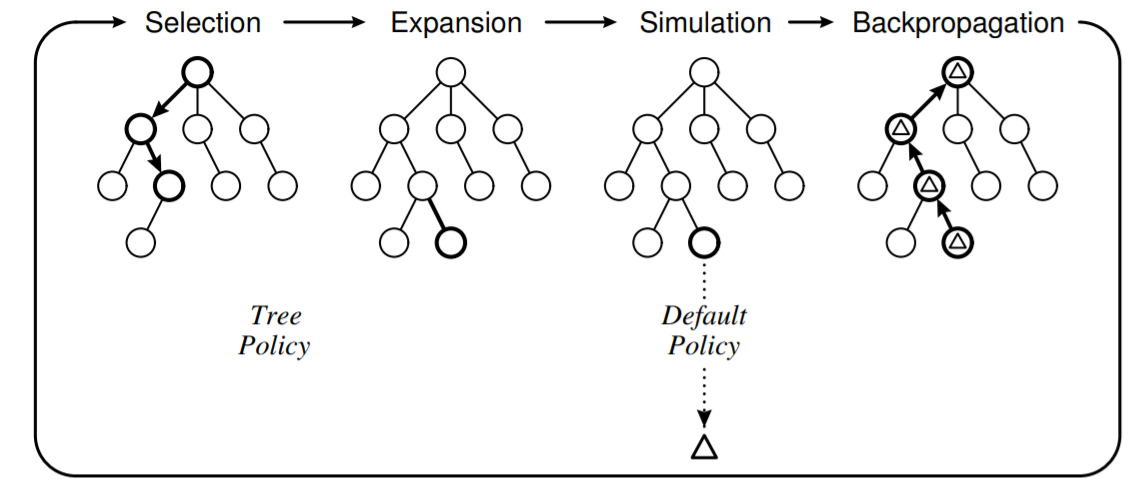
\includegraphics[scale = 0.3]{MCTS stages.png}
			\caption{One iteration of the general MCTS approach[2]}
		\end{figure}
	
		To make the above framework works, the policy of each step is crucial. The first algorithm Heuristic Monte Carlo Tree Search, a.k.a HMCTS, is a nice try based on it.
		
		\subsection{HMCTS algorithm}
		
		The general algorithm pseudocode is as follows
		
		\begin{algorithm}[H]
			\caption{HMCTS algorithm}
			\begin{algorithmic}[1]
				\Require original state $s_0$, Heuristic Knowledge $h$
				\Ensure action $a$ with the highest value of MCTS
				\State Get possible moves set $M$ of state $s_0$
				\For{move $m$ in $M$}
					\State $R_m \gets 0$
					\While{simulation times $t$ < $T$}
						\State $R_m \gets R_m + Simulation(f(s_0, m), h)$
						\State $t \gets t + 1$
					\EndWhile
					\State add $(m, R_m)$ into data
				\EndFor
				
				\State \textbf{return} action $m^\star = \mathop{\arg\max}\limits_{m \in M} R_m$
			\end{algorithmic}
		\end{algorithm}
	\begin{algorithm}[H]
		\caption{Simulation}
		\begin{algorithmic}[1]
			\Require Original state $s_0$, Heuristic Knowledge $h$
			\Ensure Reward of this state $R$
			\If{$s_0$ is terminal}
				\If{$s_0$ is win}
					\State \textbf{return} 1.0
				\ElsIf{$s_0$ is lose}
					\State \textbf{return} 0.0
				\Else
					\State \textbf{return} 0.5
				\EndIf
			\EndIf
			\If{$s_0$ satisfies $h$}
				\State obtain forced move $a$
				\State $s_{t + 1} \gets f(s_0, a)$
			\Else
				\State get possible moves set $M$
				\State randomly choose one action $a$ from $M$
				\State $s_{t + 1} \gets f(s_0, a)$
			\EndIf
			\State \textbf{return} Simulation($s_{t + 1}$, $h$)
		\end{algorithmic}
	\end{algorithm}
	
	Where $f$ is a function of the board, given state $s$ and action $a$ to attain the new state $s_{new}$.
	
	\subsection{Heuristic Knowledge}
	
	Inherent from check mate function (or seek must) function in our last check point, the Heuristic Knowledge is a simple policy for AI to check wether there are some steps it must take. During the whole \textit{Simulation} routine, if we choose every step randomly, we will easily run into some cases that is unreasonable, such as letting the opponent win from a single block four threat. To simply prune these unreasonable occasions, we have the following rules:
	\begin{itemize}
		\item If we have a chance to win, we must take it
		\item If opponent have a chance to win, we must try to block it
		\item If we have a chance to make four-in-a-row, we will make it
		\item If the opponent have a chance to make four-in-a-row, we simply block it
	\end{itemize}

	Moreover, in the following part, we will take another kind of heuristic knowledge, which is the scoring technics in our Alpha-Beta Pruning, to heuristically shrink the state space of each round of simulation.

	\subsection{Scoring the board}
	
	The score table for each pattern just goes like below
	
	\begin{table}[H]
		\setlength\tabcolsep{3pt}
		\begin{center}
			\scalebox{0.8}{
				\begin{tabularx}{10cm}{ccc}
					\toprule
					\textbf{Pattern Type} & \textbf{Definition} & \textbf{Value}\\
					\midrule
					FIVE 
					&\begin{minipage}[b]{0.3\columnwidth}
						\centering
						\raisebox{-.5\height}{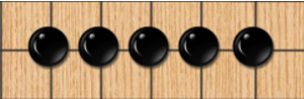
\includegraphics[width=\linewidth]{five.png}}
					\end{minipage}
					& 10000000 \\
					\midrule
					FOUR & \begin{minipage}[b]{ 0.3\columnwidth}
						\centering
						\raisebox{-.5\height}{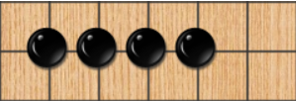
\includegraphics[width=\linewidth]{4.png}}
					\end{minipage} & 100000 \\
					\midrule
					BLOCKED\_FOUR & \begin{minipage}[b]{ 0.3\columnwidth}
						\centering
						\raisebox{-.5\height}{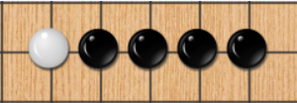
\includegraphics[width=\linewidth]{b4.png}}
					\end{minipage} & 10000 \\
					\midrule
					THREE & \begin{minipage}[b]{ 0.3\columnwidth}
						\centering
						\raisebox{-.5\height}{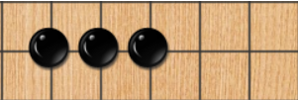
\includegraphics[width=\linewidth]{3.png}}
					\end{minipage} & 1000 \\
					\midrule
					BLOCKED\_THREE & \begin{minipage}[b]{ 0.3\columnwidth}
						\centering
						\raisebox{-.5\height}{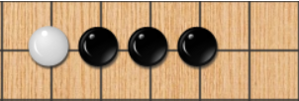
\includegraphics[width=\linewidth]{b3.png}}
					\end{minipage} & 100 \\
					\midrule
					TWO &\begin{minipage}[b]{ 0.3\columnwidth}
						\centering
						\raisebox{-.5\height}{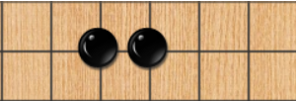
\includegraphics[width=\linewidth]{2.png}}
					\end{minipage} & 100 \\
					\midrule
					BLOCKED\_TWO & \begin{minipage}[b]{ 0.3\columnwidth}
						\centering
						\raisebox{-.5\height}{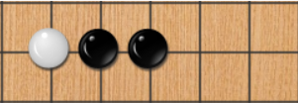
\includegraphics[width=\linewidth]{b2.png}}
					\end{minipage} & 10 \\
					\midrule
					ONE & \begin{minipage}[b]{ 0.3\columnwidth}
						\centering
						\raisebox{-.5\height}{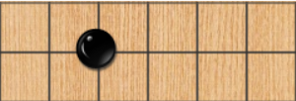
\includegraphics[width=\linewidth]{1.png}}
					\end{minipage} & 10 \\
					\midrule
					BLOCKED\_ONE & \begin{minipage}[b]{ 0.3\columnwidth}
						\centering
						\raisebox{-.5\height}{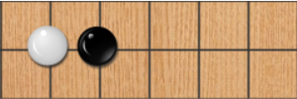
\includegraphics[width=\linewidth]{b1.png}}
					\end{minipage} & 1 \\
					\bottomrule
				\end{tabularx}
			}
			\caption{Score For Each Pattern}
			\label{tab:table1}
		\end{center}
	\end{table}
	
	The score of a move is evaluated based on how well it attack and how much it weaken the opponent. Here We divide dots into two categories, empty points and colored points.
	
	For assigning a value to a colored point, we use the radius of 6 grid, scan its horizontal(h), vertical(v), and diagonal directions(d1/d2). Calculate patterns with the same color formed in each direction respectively, and take the largest in that direction. Finally, sum up the scores in the four directions to get a colored point score.
	
	For assigning a value to a empty point, we assume it's black and white and calculate the score respectively. Thus it has a positive white score for the enemy and black score for AI player.
	\begin{figure}[H]
		\centering
		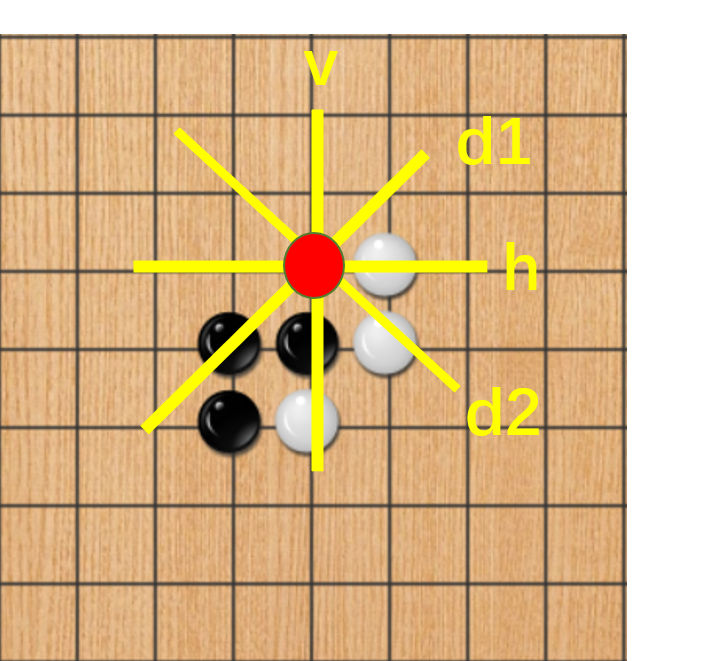
\includegraphics[scale=0.4]{example.png}
		\caption{An example of evaluating an empty point }
		\label{figure}
	\end{figure}
	In this example the white score of red point is:
	$$
	\begin{small}
		\begin{aligned}
			S_{white} =& S_{TWO}\times 2+S_{BLOCK\_ONE}\times 2\\ &= 100\times 2+1\times 2\\ &= 202
		\end{aligned}
	\end{small}
	$$
	Besides, the black score of red point is:
	$$
	\begin{small}
		\begin{aligned}
			S_{black} &= S_{BLOCK\_TWO}+S_{TWO}+S_{BLOCK\_ONE}\times 2\\ &= 10+100+1\times 2\\ &= 112
		\end{aligned}
	\end{small}
	$$
	
	We also inherent all the quick update strategy in Alpha-Beta Pruning to avoid too much cost on the simulation step.
	
	\subsection{UCT algorithm}

	As we mentioned in introduction, HMCTS algorithm has a large drawback that there is a huge work load for personal computer to provide point estimator of winning rate of each move. So here in UCT algorithm, we use a confidence interval to upper bound the estimator, which could have a better trade-off between "exploration and exploitation". The routine will be like that
	
	\begin{algorithm}[H]
		\caption{UCT algorithm}
		\begin{algorithmic}[1]
			\Require original state $s_0$, Heuristic Knowledge $h$
			\Ensure action $a$ with the highest value of UCT
			\While{within computational budget}
				\State $m \gets Tree policy(s_0)$
				\State $r \gets Simulation(f(s_0, m), h)$
				\State Update($m$, $r$)
			\EndWhile
			\State \textbf{return} BestMove($s_0$)
		\end{algorithmic}
	\end{algorithm}

	\begin{algorithm}[H]
		\caption{Treepolicy}
		\begin{algorithmic}[1]
			\Require original state $s_0$
			\Ensure Act $m$
			\State Get possible moves set $M$
			\If{$M$ hasn't been fully expanded}
				\State \textbf{return} any unexpanded move $m$
			\Else
				\State \textbf{return} BestMove($s_0$)
			\EndIf
		\end{algorithmic}
	\end{algorithm}
	
	\begin{algorithm}[H]
		\caption{BestChild}
		\begin{algorithmic}[1]
			\Require original state $s_0$
			\Ensure best move $m^\star$ of state $s_0$
			\State Get possible moves set $M$
			\State \textbf{return} $\mathop{\arg \max}\limits_{m \in M}\frac{Q(m)}{N(m)} + c\sqrt{2\frac{\ln N(m)}{N}}$
		\end{algorithmic}
	\end{algorithm}

	\begin{algorithm}[H]
		\caption{Update}
		\begin{algorithmic}[1]
			\Require move $m$ and its reward in one round of simulation $r$
			\State $Q(m) \gets Q(m) + r$
			\State $N(m) \gets N(m) + 1$
			\State $N \gets N + 1$
		\end{algorithmic}
	\end{algorithm}
	
	In the simulation of UCT, we also expand and choose the child node with maximum UCB value.
	
	To show the advantage of UCT, we will take a glimpse at the origin of them, the Multi-Armed Bandit scenario in the next section.
	
	\end{multicols}
	
	\begin{multicols}{2}
		[
		\section{Multi-Armed Bandit}
		Multi-Armed Bandit (MAB) is a famous scenario in online learning, it's basic setting is in each round, we could check one arm of the bandit, and receive corresponding reward due to an unkown distribution (\textit{stochastic bandit} setting). Our goal is to find the best arm, or in online learning, minimize our expect regret. We will show two algorithms of this problem, ETC and UCB algroithm, which could be translate into HMCTS and UCT algorithm. Moreover, we will show some analysis of them (due to the page limit, we will not show the proof of it, you could find them in our reference).
		]
		
		\newpage
		\subsection{ETC algorithm}
		
		The easiest idea of this problem is, we simply try each arm several times to give an estimator of it's expect.
		
		To analyze this algorithm, we shuold take a look at the word "regret". In stochastic bandit setting, regret means
		
		\begin{equation*}
			\begin{split}
				\operatorname{Regret}_{T}& :=\mathbb{E}\left[\sum_{t=1}^{T} g_{t, A_{t}}\right]-\min _{i=1, \ldots, d} \mathbb{E}\left[\sum_{t=1}^{T} g_{t, i}\right]\\
				&=\mathbb{E}\left[\sum_{t=1}^{T} g_{t, A_{t}}\right]-\min _{i=1, \ldots, d} d\mu_{i}
			\end{split}
		\end{equation*}
		
		
		Then in [3][4] we know the analysis for it's regret is (under some mild assumption)
		
		\begin{equation*}
			\operatorname{Regret}_{T} \leq m \sum_{i=1}^{d} \Delta_{i}+(T-m d) \sum_{i=1}^{d} \Delta_{i} \exp \left(-\frac{m \Delta_{i}^{2}}{4}\right)
		\end{equation*}
		
		We could see that inside this upper bound, we need the actual knowledge of gaps $\Delta_i$ to tunning parameter $m$ for optimal bound, which is unreasonable in this setting beacuse it makes this problem completely trivial.
		
		This algorithm is not completely the same as HMCTS, but we could see the left term in the upper bound as the cost for exploration of new moves. This idea is almost the same in HMCTS, we need to pay somthing to search for the best arm, which leads to more regret in exploration term.
		
		\begin{algorithm}[H]
			\caption{ETC algorithm}
			\begin{algorithmic}[1]
				\Require $T, m \in \mathbb{N}, 1 \leq m \leq \frac{T}{d}$
				\State $S_{0, i} = 0, \hat{\mu_{0, i}} = 0, i = 1, 2, \ldots, d$
				\State $t = 1$
				\For{$t \leq T$}
				\State Choose $A_t = \begin{cases}
					(t mod d) + 1 & t \leq dm \\
					\mathop{\arg \max} \hat{\mu_{dm, i}} & t > dm
				\end{cases}$
				\State Observe $g_{t, A_t}$
				\State $S_{t, i} = S_{t - 1, i} + \mathbf{1}[A_t = i]$
				\State $\hat{\mu}_{t, i}=\frac{1}{S_{t, i}} \sum_{j=1}^{t} g_{j, A_{j}} \mathbf{1}\left[A_{j}=i\right], i=1, \ldots, d $
				\State $t = t + 1$
				\EndFor
			\end{algorithmic}
		\end{algorithm}
		
		\subsection{UCB algorithm}
		
		The drawback of the ETC algorithm is that it can not has a good balance between exploration and exploitation without knowledge of gaps $\Delta_i$. To modify this disadvantage, we could change our estimation of one arm from point estimation to confidence interval. That is to say, we balance exploration, which we try to figure out which arm is good, and exploitation, that means we use the selected arm to gain reward, in a dynamic way. Because confidence interval means with enough rounds of exploration, we could bound the actual expect reward of one arm with a probability. By comparing the upper confidence bound, we could have a smooth transition between exploration and exploitation (without tunning the exploration phase like ETC does). Here is the pseudocode of it
		
		\begin{algorithm}[H]
			\caption{UCB algorithm}
			\begin{algorithmic}[1]
				\Require $\alpha > 2, T \in \mathbb{N}$
				\State $S_{0, i}=0, \hat{\mu}_{0, i}=0, i=1, \ldots, d$
				\For{$t < T$}
					\State $A_{t}=\mathop{\arg \max}\limits_{i=1, \ldots, d} \begin{cases}\mu_{t-1, i}+\sqrt{\frac{2 \alpha \ln t}{S_{t-1, i}}} & S_{t-1, i} \neq 0 \\ -\infty & \text { otherwise }\end{cases}$
					\State Observe $g_{t, A_t}$
					\State $S_{t, i}=S_{t-1, i}+\mathbf{1}\left[A_{t}=i\right]$
					\State $\hat{\mu}_{t, i}=\frac{1}{S_{t, i}} \sum_{j=1}^{t} g_{t, A_{t}} \mathbf{1}\left[A_{t}=i\right], i=1, \ldots, d$
				\EndFor
			\end{algorithmic}
		\end{algorithm}
	
	Under some mild assumption, we have the following two bounds for UCB
	
	\begin{equation*}
		\begin{split}
			\operatorname{Regret}_{T} & \leq \frac{\alpha}{\alpha-2} \sum_{i=1}^{d} \Delta_{i}+\sum_{i: \Delta_{i}>0} \frac{8 \alpha \ln T}{\Delta_{i}} \\
			\operatorname{Regret}_{T} & \leq 4 \sqrt{2 \alpha d T \ln T}+\frac{\alpha}{\alpha-2} \sum_{i=1}^{d} \Delta_{i}
		\end{split}
	\end{equation*}

	So compare bounds in ETC and UCB we could see that, without any knowledge of gaps $\Delta_i$, the UCB could achieve the same asymptotic expect regret bound as UCT.
	\end{multicols}
	
	\newpage
	
	\begin{multicols}{2}
		[
		\section{Optimization}
		]
		
		\subsection{Node structure}
		
		We construct the $Node$ data structure to store UCB value of each stage, number of visit, parent, child and player information. With the aid of this data structure, we could construct our MCT tree, and lay a firm fundation for optimization following.
		
		\subsection{$\epsilon$-Greedy}
		
		In our simulation, it is easy to see that we greedily choose the child node with biggest UCB value, this policy make sense in the first glance, however, in fact, the simulation process is just an approximation to the real world, which means both of the players takes the same policy we imagine, and this policy even not that make sense as we did in Alpha-Beta pruning (we sacrifice some of them for quicker simulation). Therefore, continuing select the son with biggest UCB value might cause so-called "Over-fitting", the win rate approximation might perform too good for the given policy, but might perform way worse than the real world. So we import $\epsilon$-greedy method, by selecting some other moves randomly with a probability. Which could effectively avoid the case the AI being trapped inside the given simple policy. In our implementation we take the following type of move selection policy
		
		\begin{equation*}
			\pi^{\epsilon}(s)=\left\{\begin{array}{cc}
				a, & P = \frac{\varepsilon}{|A|} \\
				\underset{a}{\operatorname{argmax}}  UCB(a), & P = 1-\varepsilon
			\end{array}\right.
		\end{equation*}
	
		In our program $|A|$ means the number of moves in structure $activemove$. After we import this selection policy, we see a prominent improve in performance.
		
		\subsection{Quick activemove update \& withdraw}
		
		In our last report, we conclude one future work, which is quickly update the active move in each alter on board. This time we implement the $add\_move$ module, inside the module, we update the active move for just searching the area near our new move to check if there are something new could be added inside, which avoid scanning the whole board everytime we change the board. This optimization highly acclerating our algorithm.
		
		We also import some optimization in the withdraw module, which is a more tricky optimization. As all the active moves in the parent node will be expanded, so we could simply recover the active move by taking all the brother nodes and this node inside the activemove structure to recover it to the previous stage.
		
	\end{multicols}
	\begin{multicols}{2}
		[
		\section{Experiments}
		]
		
		\begin{tabular}{|c|c|c|c|}
			\hline$-$ & mix1 & & mix1\\
			\hline \hline pisq7 & $0: 12$ & Yixin2018 & $0: 12$ \\
			\hline \hline Noesis & $0: 12$ & Eulring & $1: 11$ \\
			\hline \hline Wine18 & $0: 12$ & valkyrie & $6: 6$\\
			\hline \hline Sparkle & $0: 12$ & fiverow & $6: 6$ \\
			\hline \hline zetor2017 & $0: 12$ & PureRocky & $6: 6$ \\
			\hline \hline pela & $0: 12$ & mushroom & $11: 1$ \\
			\hline
		\end{tabular}
	
	 	We could see that our AI could easily defeat MUSHROOM, and could match PUREROCKY, FIVEROW, VALKYRIE. Obviously it works not as good as Alpha-Beta Pruning because to make the whole frame work work better, it needs some help from neural network for better policy (which is what AlphaGO did). But actually in future work section, we still got some more jobs to do.
	 	
	\end{multicols}

	\begin{multicols}{2}
		[
		\section{Future work}
		]
		
		\subsection{Natural Selection}
		
		Notice that we have plenty of parameters inside our program, the job of tunning is laborious. But we could use a natrual selection way, to autonomous tunning the parameters. We simply set up some battle between current AIs, kill the AI that lose the game and generate new AIs from the winner. In the process we could involve some survival pressure and variation for better performance.
		
		\subsection{Policy network \& Value network}
		
		In the work of AlphaGo we could easily see that they take advantage of neural network to support their MCTS, and using reinforcement learning to adjust all the parameters inside networks[5]. At this time we are not equipped with knowledge of neural network, but with some knowledge of reinforcement learning, we are looking forward to apply some of the strategy from it to GOMOKU in next check point, and maybe obtain some idea from the neural network background.
		
	\end{multicols}

	\begin{thebibliography}{99}
		\bibitem{ref1} Zhentao Tang, Zhao, D., Kun Shao, Le Lv. (2016). ADP with MCTS algorithm for Gomoku. 2016 IEEE Symposium Series on Computational Intelligence (SSCI).
		\bibitem{ref2} C. B. Browne, E. Powley, D. Whitehouse, S. M. Lucas, P. I. Cowling, P. Rohlfshagen, S. Tavener, D. Perez, S. Samothrakis, and S. Colton, "A Survey of Monte Carlo Tree Search Methods," IEEE Transactions on Computational Intelligence and AI in Games, vol. 4, pp. 1-43, 2012.
		\bibitem{ref3} Francesco Orabona, "A Modern Introduction to Online Learning"
		\bibitem{ref4} Tor Lattimore and Csaba Szepesvári, "Bandit Algorithms", Cambridge University Press
		\bibitem{ref5} Chang, H.S., M.C. Fu, J. Hu, and S.I. Marcus. 2016. “Google Deep Mind’s AlphaGo”. OR/MS Today.
	\end{thebibliography}
	%------------------------------------------------
	
	%----------------------------------------------------------------------------------------
	%	REFERENCE LIST
	%----------------------------------------------------------------------------------------
	
	% \cite{Bird2014}
	% \printbibliography
	
	%----------------------------------------------------------------------------------------
	
\end{document}
